\chapter[Resultados Obtidos]{Resultados Obtidos}

Este capítulo visa relatar os resultados obtidos em ambas as coletas de opinião
realizadas para verificar a validades das hipóteses propostas neste trabalho.
Dessa forma, cada coleta será analisada em uma seção própria.

Vale ressaltar que ambas as coletas de dados foram realizadas com graduados e
graduandos do curso de Engenharia de Software da Universidade de Brasília. Além
disso, permitiu-se a coleta para qualquer usuário com sistemas Debian ou
derivados do mesmo.

\section{Primeira coleta de opinião}

A primeira coleta de opinião foi realizada com 10 pessoas, onde para cada
pessoa foram analisadas três estratégias de recomendação, sendo elas:

\begin{itemize}
    \item \textbf{cbh:} Estratégia baseada em conteúdo, onde metade do
    perfil do usuário é formado por \textit{Debtags} e a outra metade por termos
    da descrição dos pacotes. Tanto as \textit{Debtags} e os termos são definidos
        utilizando a técnica do \textit{TFIDF};
    \item \textbf{cbtm:} Estratégia baseada em conteúdo utilisando o contexto
    temporal, assim como na estratégia `cbh`, o perfil do usuário é composto
    por duas metades, sendo as \textit{Debtags} e os termos da descrição dos pacotes,
    porém eles são definidos através de dois pesos, sendo o primeiro uma
    análise de quais pacotes foram recentemente utilizados, e o segundo peso
    se trata da utilização do \textit{TFIDF};
    \item \textbf{cbml:} Estratégia baseada em conteúdo, onde o perfil do
    usuário é formado tanto por \textit{Debtags} quanto termos, porém não é composto
    por metade de cada um, utilizando esse perfil é realizado a
    recomendação de vários pacotes. Então é utilizado o algoritmo de
    aprendizado de máquina para identificar quais dentre esses pacotes
    devem ser recomendados.
\end{itemize}

Dentre as estratégias a `cbh` já estava implementada no AppRecommender, e as
estratégias `cbtm` e `cbml` se tratam das estratégias implementadas afim de
testar as hipóteses desta pesquisa.

Para cada estratégia foram selecionadas as 10 melhores recomendações
e essas foram ordenadas em ordem alfabética e apresentadas uma a uma para
o usuário realizar a pontuação, como foi descrito anteriormente.

A coleta de dados apresentou os resultados apresentados na Figura
\ref{fig:primeiro_experimento}

\pagebreak

\begin{figure}[h]
  \centering
  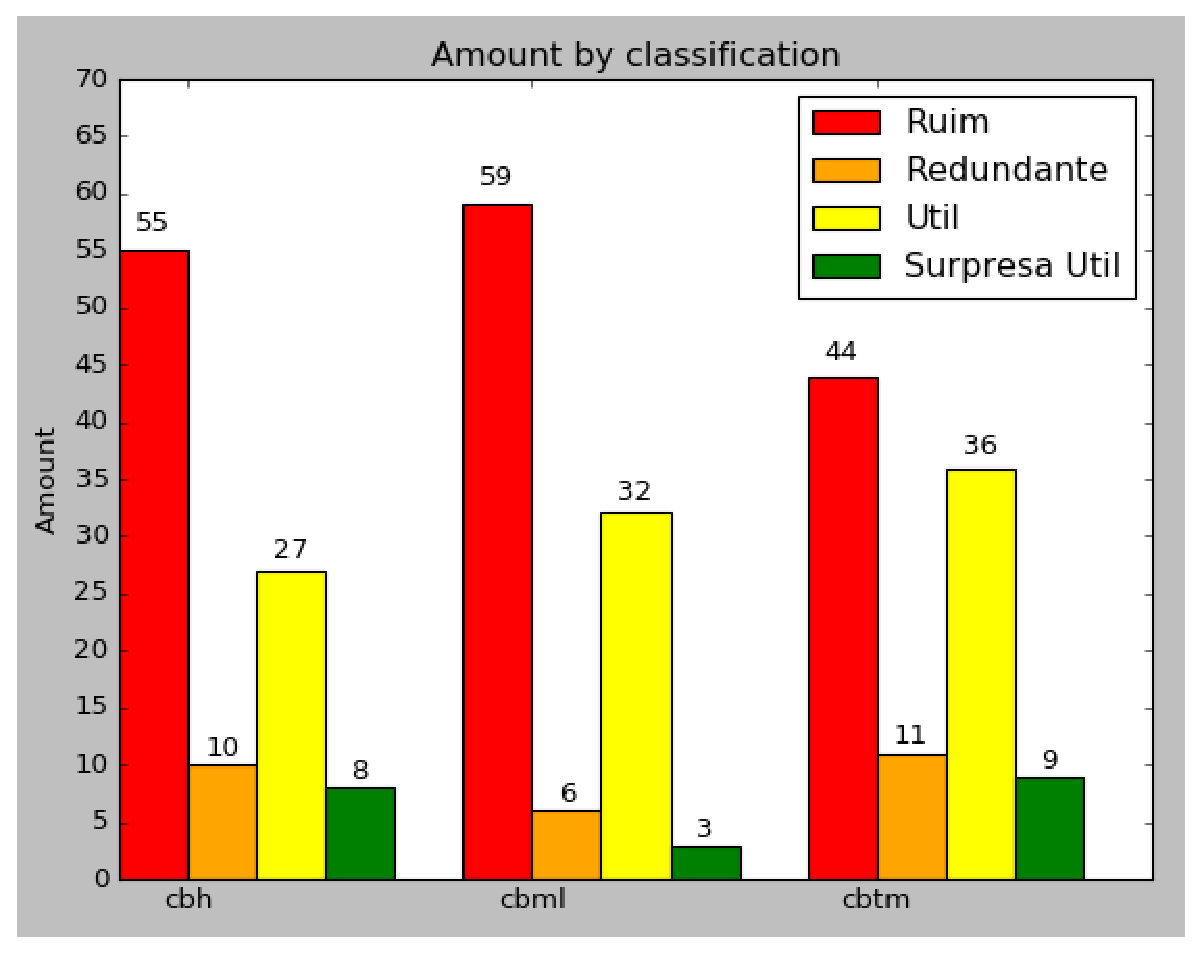
\includegraphics[width=0.9\textwidth]{figuras/primeiro_experimento.eps}
  \caption{Resultados da primeira coleta de opinião}
  \label{fig:primeiro_experimento}
\end{figure}

Analisando os dados coletados pode-se observar que os indices de recomendações
ruins das estratégias `cbh` e `cbml` foram maiores que os índices da estratégia
`cbtm`, e também é notável a diferença entre recomendações úteis e surpresas
boas, pois a estratégia `cbtm` possui 45 recomendações nessas classificações
enquanto as estratégias `cbml` e `cbh` possuem 35.

Através dos dados coletados observa-se que mesmo a estratégia `cbtm` possuindo
um pouco de destaque, todas as estratégias aprensentaram um índice muito alto
de recomendações ruins

O gráfico apresentado na Figura \ref{fig:metricas_segundo_experimento} mostra
a análise das métricas propostas na Seção \ref{sec:estudo_usuario}, que são:
precisão, novidade e ruim.

\pagebreak

\begin{figure}[h]
  \centering
  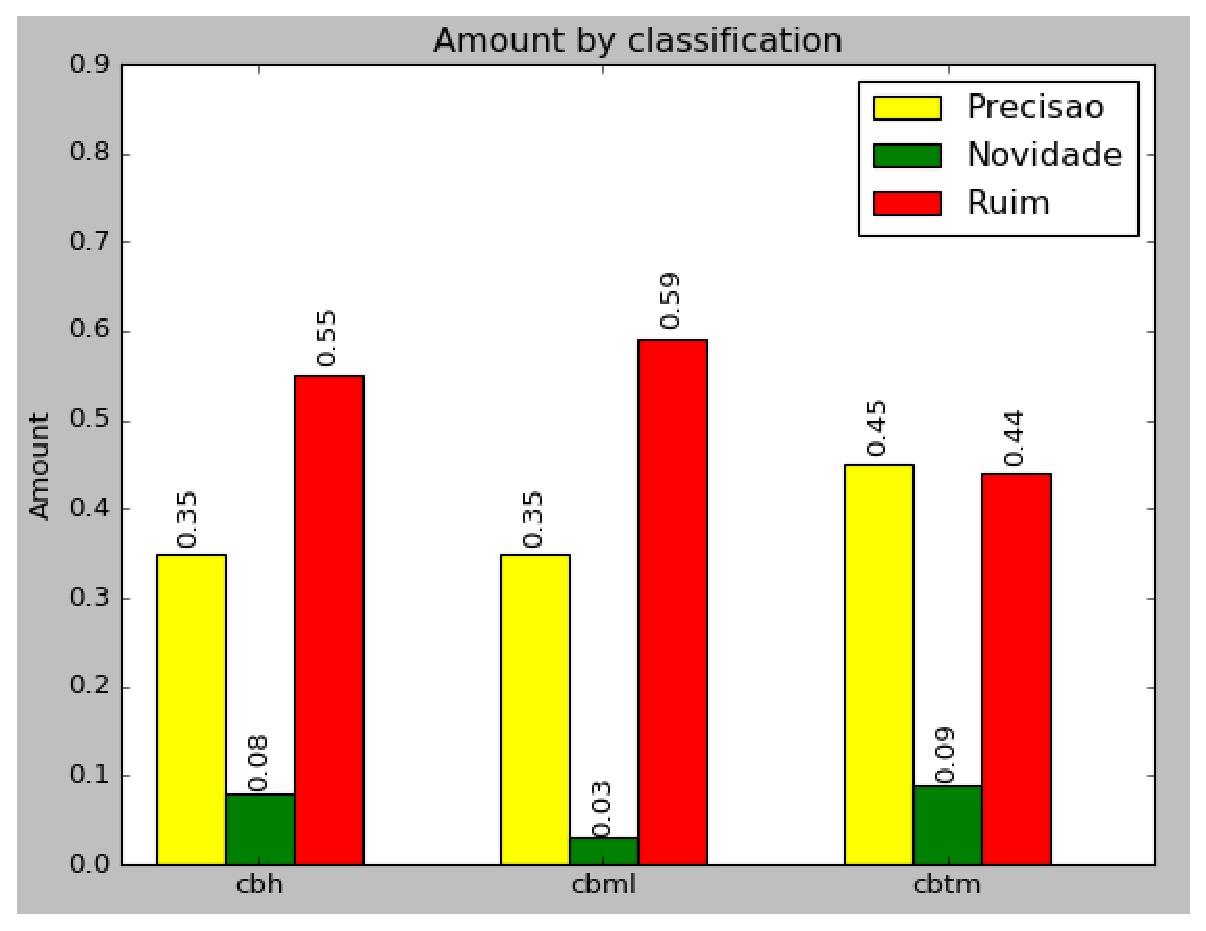
\includegraphics[width=0.9\textwidth]{figuras/metricas_primeiro_experimento.eps}
  \caption{Métricas da primeira coleta de opinião}
  \label{fig:metricas_primeiro_experimento}
\end{figure}

Analisando a precisão e a novidade de cada recomendação, na Figura
\ref{fig:metricas_segundo_experimento}, observa-se que a estratégia que
apresentou melhores resultados embora por pouca diferença, foi a estratégia
`cbtm`, fato que pode demonstrar que a estratégia determinística se saiu melhor
que a estratégia de aprendizado de máquina, para esses usuários que
participaram da primeira coleta. A Tabela \ref{tab:resultado_p1} resume os
resultados das métricas encontradas:

\begin{table}[]
    \centering
    \begin{tabular}{|l|l|l|l|}
    \hline
    & \textbf{Precisão} & \textbf{Novidade} & \textbf{Ruim} \\ \hline
    \textbf{cbh}  & 0.35     & 0.08     & 0.55 \\ \hline
    \textbf{cbtm} & 0.35     & 0.03     & 0.59 \\ \hline
    \textbf{cbml} & 0.45     & 0.09     & 0.44 \\ \hline
    \end{tabular}
    \caption{Resultados das métricas da primeira coleta de opnião}
    \label{tab:resultado_p1}
\end{table}

Através dos dados coletados foi analisado a métrica \textit{PorcentagemAcertos}
para a estratégia `cbml` através da validação cruzada, onde o resultado dessa
métrica é de apenas 22,87\%, resultado obtido pela média do valor apresentado
por essa métrica para cada usuário, esse valor de 22,87\% indica que os
resultados das recomendações não são exatamente o que se espera pela técnica
do cross validation, o que demonstra que até a próxima coleta de opinião deve ser
realizado melhorias quanto ao tratamento dos dados, como a definição do perfil
do usuário, que pode ser melhorado afim de que os resultados dessa métrica
possam ser melhorados.

Os resultados dessa primeira coleta não foram o que os pesquisadores desse
projeto esperavam, pois esperava-se que os resultados obtidos tivessem um
resultado mais satisfatório quanto a qualidade das recomendações, porém, essa
primeira coleta de opinião foi executada com o objetivo de coletar dados afim de
compreender mais sobre o perfil dos usuários e o que estava sendo recomendado,
e então utilizar isso para melhorar o sistema de recomendação e posteriormente
realizar uma segunda coleta de opinião, onde de fato o objetivo é comparar qual
estratégia se saiu melhor.

\section{Segunda coleta de opinião}

Dado os resultados da primeira coleta de opinião, as seguinte medidas foram tomadas
para a segunda coleta de opinião:

\begin{itemize}
   \item \textbf{Mudar cálculo do contexto temporal de um pacote: } Visto que
   pela primeira coleta, o contexto temporal do pacote não estava
   refletindo bem os usos do usuário. Isso percebido por analisar as informações
   temporais do \textit{popularity-contest} junto com os arquivos usados pela
   abordagens desta pesquisa para realizar o cálculo do contexto temporal.
   Percebeu-se que não seria ideal apenas verificar por pacotes com
   arquivos binários, mas sim por qualquer pacote que forneça alguma
   biblioteca também. Dessa forma, o cálculo do contexto temporal de um
   pacote foi atualizado. O contexto temporal de um pacote agora é calculado de
   forma semelhante ao obtido pelo \textit{popularity-contest}, onde o tempo de
   acesso de cada arquivo relacionado a um pacote é observado e o maior tempo
   encontrado é considerado o tempo de acesso.

   \item \textbf{Balancear rótulo dos pacotes: } Com o intuito de melhorar
   a acurácia dos algoritmos de aprendizado de máquina, resolveu-se melhor
   balancear os pacotes do usuário. Para isso, os pacotes são ordenados pelo seu
   contexto temporal e dividos em três grupos de igual tamanho, onde cada grupo
   representa um rótulo possível.

   \item \textbf{Selecionar pacotes apenas instalados diretamente pelo
   \textit{apt}:} Para melhorar o perfil de usuário, resolveu-se selecionar não
   mais os pacotes marcados como manualmente instalados pelo sistema, e sim
   apenas aqueles cujo usuário instalou diretamente pelo \textit{apt}.

   \item \textbf{Implementar nova forma de representar um pacote: } Para
   verificar se outras formas de representação de um pacote podem ser mais
   eficientes, implementou-se uma nova estratégia de aprendizado de máquina, que
   usa o modelo \textit{Bag Of Words} juntamente com o \textit{TFIDF} para
   representar um pacote.

   \item \textbf{Uso da estratégia de expansão de query: } Essa estratégia já
   implementada pelo \textit{AppRecommender} faz com que o \textit{Xapian}
   apenas receba os pacotes que deva fazer a pesquisa relacionada e o mesmo deve
   então ser capaz de retirar de cada pacote as informações mais importantes
   para realizar a pesquisa. Dessa forma, as estratégias de aprendizado de
   máquina também foram combinadas com essa estratégia com o intuito de
   verificar se melhores resultados foram gerados.

   \item \textbf{Diminuir número de pacotes passados para o Xapian:} Para as
   estratégias de aprendizado de máquina, apenas os pacotes marcados como
   \textit{Really Useful} (RU) são usados para criar o perfil do
   usuário. Isso se dá pelo fato de tentar reduzir o perfil do usuário para
   que o mesmo seja mais focado nos gostos atuais do usuário.

   \item \textbf{Uso da estratégia \textit{cb} ao invés da \textit{cbh}:} Para
   a primeira coleta de opinião, a estratégia \textit{cbh} foi usada. Entretanto,
   a segunda coleta quis colocar mais foco nos termos dos pacotes e
   não de forma equilibrada como funciona o \textit{cbh}. Dessa forma,
   a estratégia do \textit{AppRecommender} usada para comparação com as
   estratégias de contexto temporal, foi a estratégia \textit{cb}, que usa
   tanto termos do pacote como \textit{Debtags}, mas não garante que as mesmas
   apareçam na mesma quantidade no perfil do usuário.

   \item \textbf{Mudança de nome da estratégia \textit{cbml} para
   \textit{mlbva}:} Como agora existem duas estratégias distintas usando
   aprendizado de máquina, resolveu-se renomear a estratégia \textit{cbml}
   para \textit{mlbva}, que significa \textit{Machine Learning Binary
   Vector Approach}. Esse padrão também é seguido para a estratégia de
   \textit{Bag Of Words}, \textit{mlbow}, que significa \textit{Machine
   Learning Bag Of Words}.

   \item \textbf{Retirar pacotes que possuem dependências de programas não
   instalados no sistema do usuário:} Durante a primeira coleta de opinião, foi
   observado a recomendação de alguns pacotes relacionados a pacotes que não
   estavam presentes no sistema do usuário, como o pacote
   \textit{auto-complete-el}, que é um pacote que adiciona a funcionalida
   de auto-completar para o pacote \textit{emacs}. Entretanto, se o usuário
   não tem o pacote \textit{emacs} instalado, tal recomendação não é de
   grande ajuda. Dessa forma, pacotes que dependem de pacotes executáveis,
   só podem ser recomendados se tais dependências já estiverem instaladas
   no sistema do usuário.

\end{itemize}

Além desses pontos já citados, a segunda coleta de opinião também foi realizada com
mais usuários, 24 no total, sendo que os usuários escolhidos também apresentavam
um perfil mais geral quanto aos sistemas operacionais usados, pois para a
primeira coleta os usuários eram majoritariamente usuários Debian.

Dito, isso o resultado geral da pesquisa pode ser visto no Gráfico
\ref{fig:segundo_experimento}, onde seus \textit{labels} são respectivamente:

\begin{itemize}
    \item \textbf{mlbow}: Aprendizado de máquina com \textit{Bag Of Words}
    \item \textbf{mlbva\_eset}: Aprendizado de máquina com vetor binário e
    expansão de query.
    \item \textbf{cb}: Estratégia com perfil de usuário sem contexto temporal.
    \item \textbf{cbtm}: Estratégia deterministica com contexto temporal.
    \item \textbf{mlbva:} Aprendizado de máquina com vetor binário.
    \item \textbf{mlbow\_eset:} Aprendizado de máquina com \textit{Bag Of Words}
        usando expansão de query.
    \item \textbf{cb\_eset:} Estratégia usando apenas expansão de query, sem
        contexto temporal.
\end{itemize}

\begin{figure}[h]
  \centering
  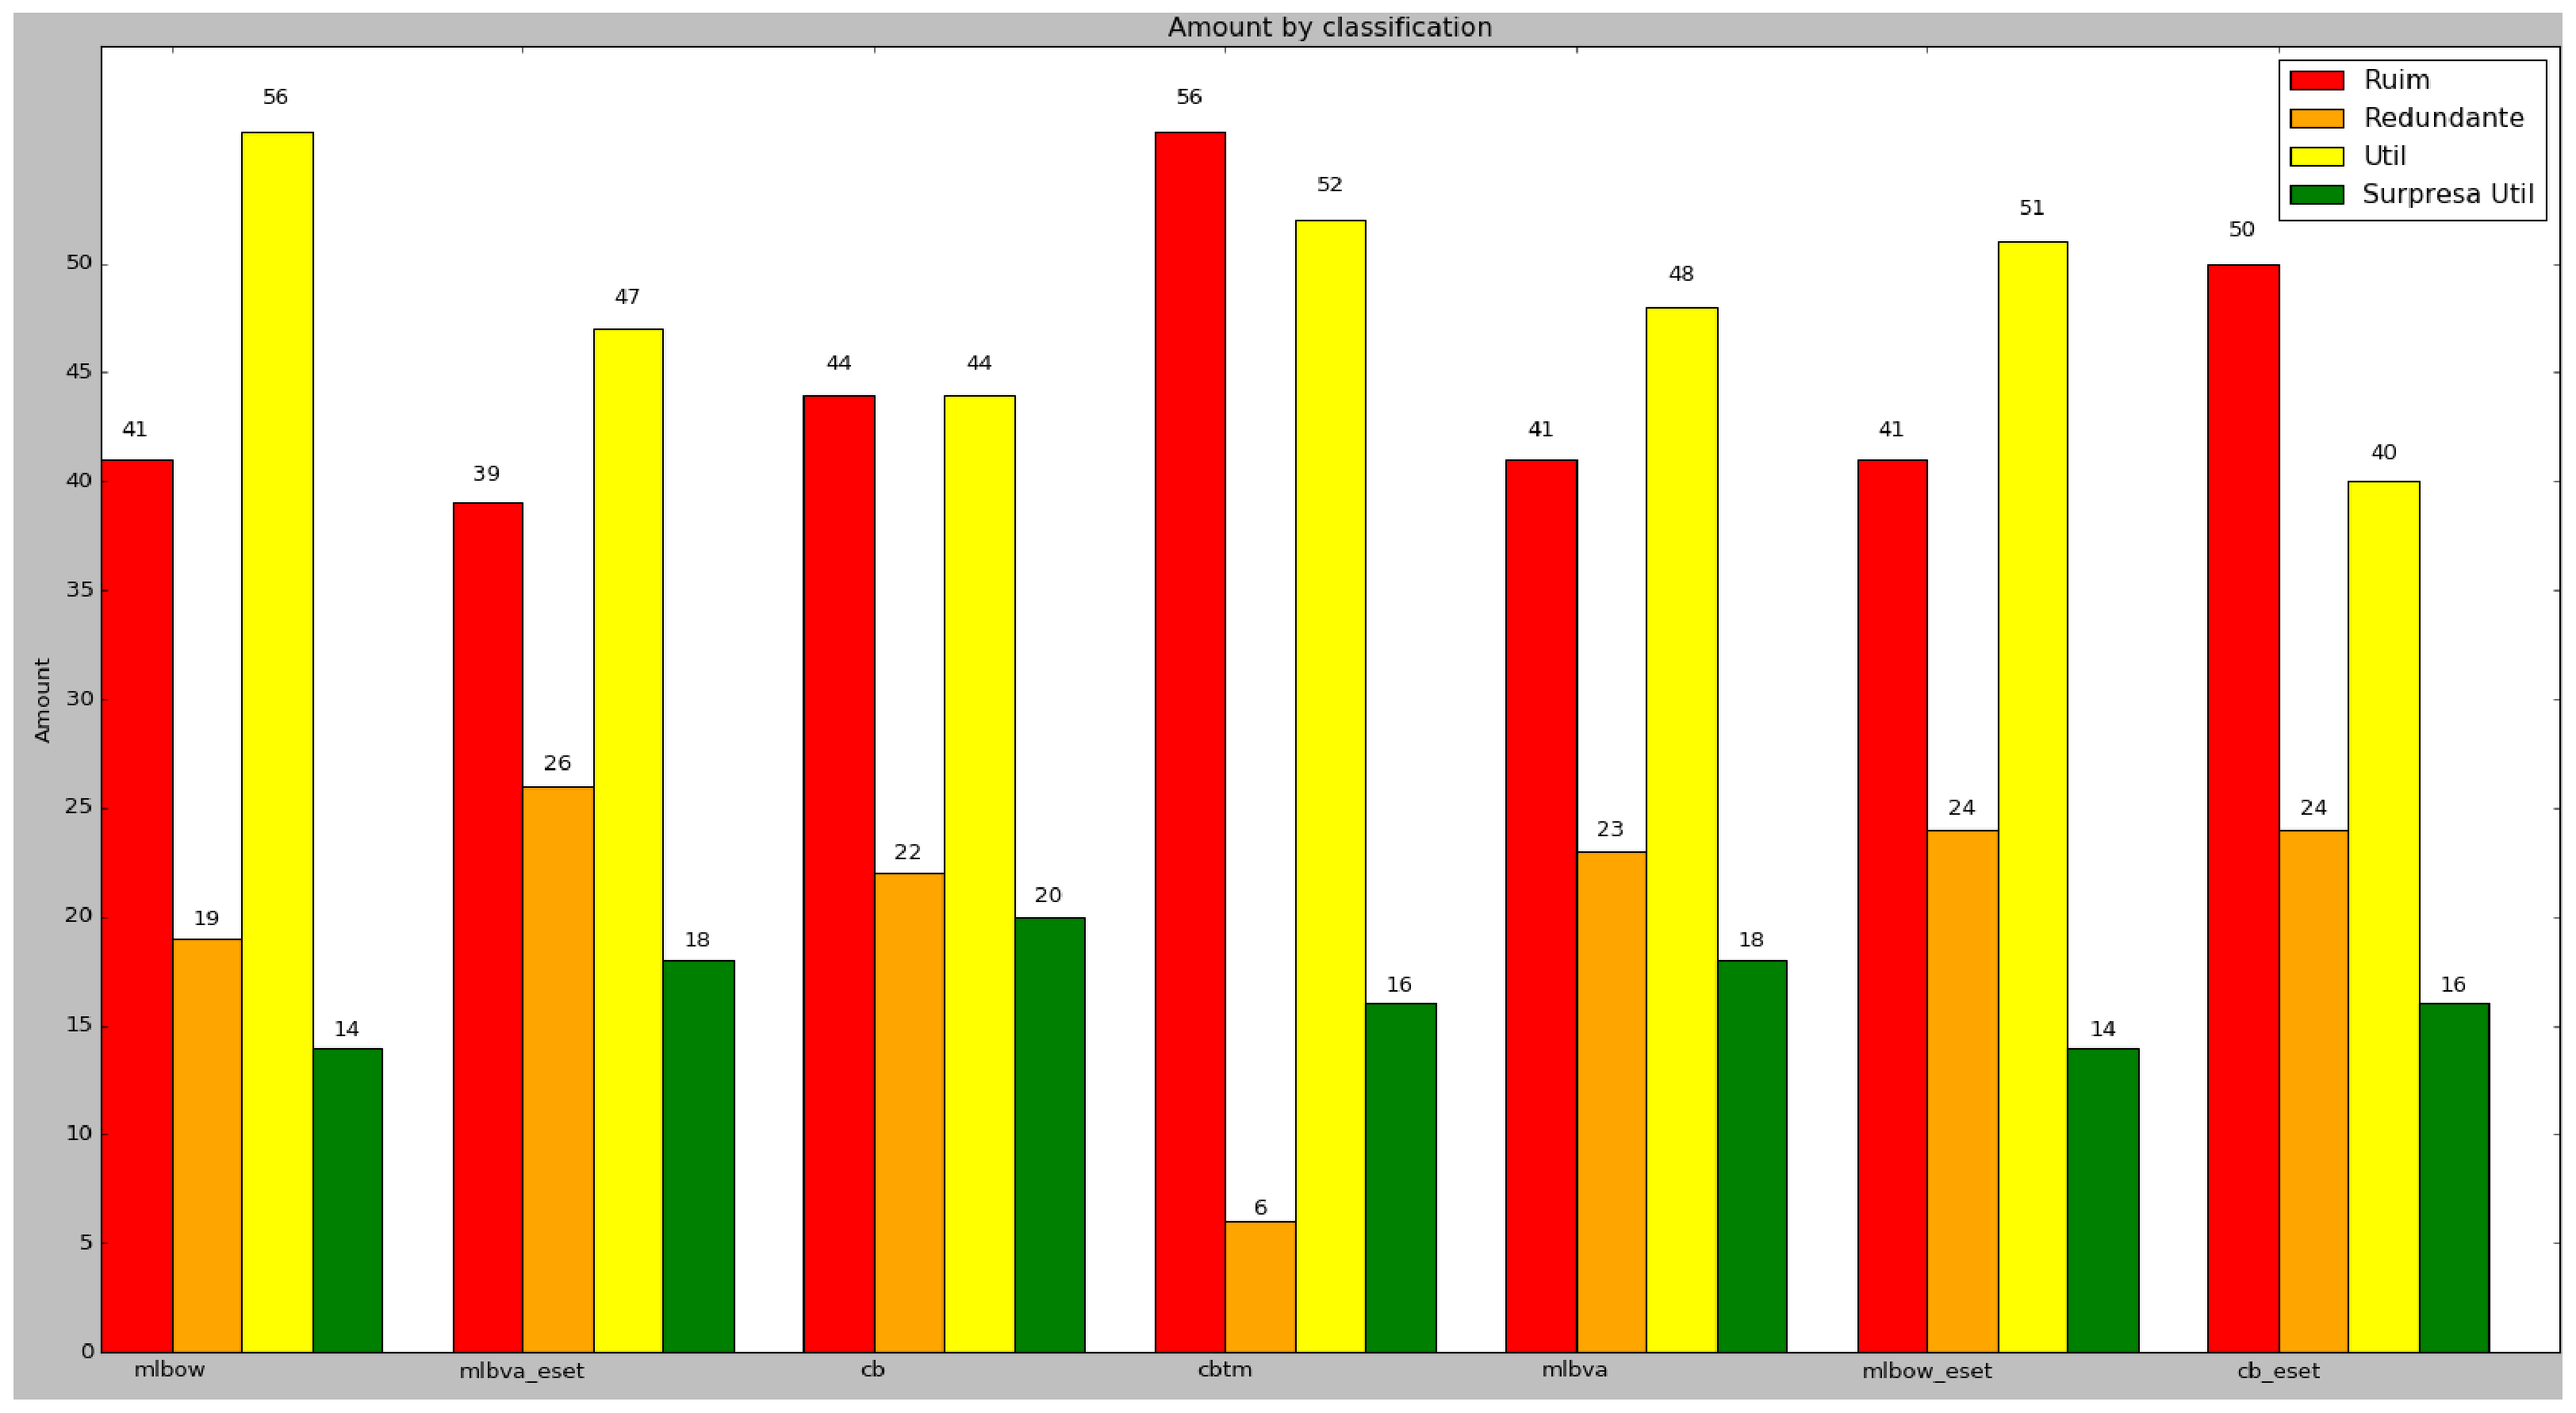
\includegraphics[width=0.9\textwidth]{figuras/segundo_experimento.eps}
  \caption{Resultados da segunda coleta de opinião}
  \label{fig:segundo_experimento}
\end{figure}

Visualmente, pode-se perceber que apenas as estratégias de aprendizado de
máquina apresentaram um total de recomendações úteis ao usuário maior que o
total de recomendações ruins. Além disso, percebe-se que as estratégias como um
todo estão produzindo poucos resultados considerados uma surpresa para usuário e
estão gerando números próximos de pacotes redundantes.

Uma melhor análise pode ser feita ao observar o Gráfico
\ref{fig:metricas_segundo_experimento} com a relação as métricas calculadas para cada
estratégia, conforme definidas na Seção \ref{sec:estudo_usuario}

\begin{figure}[h]
  \centering
  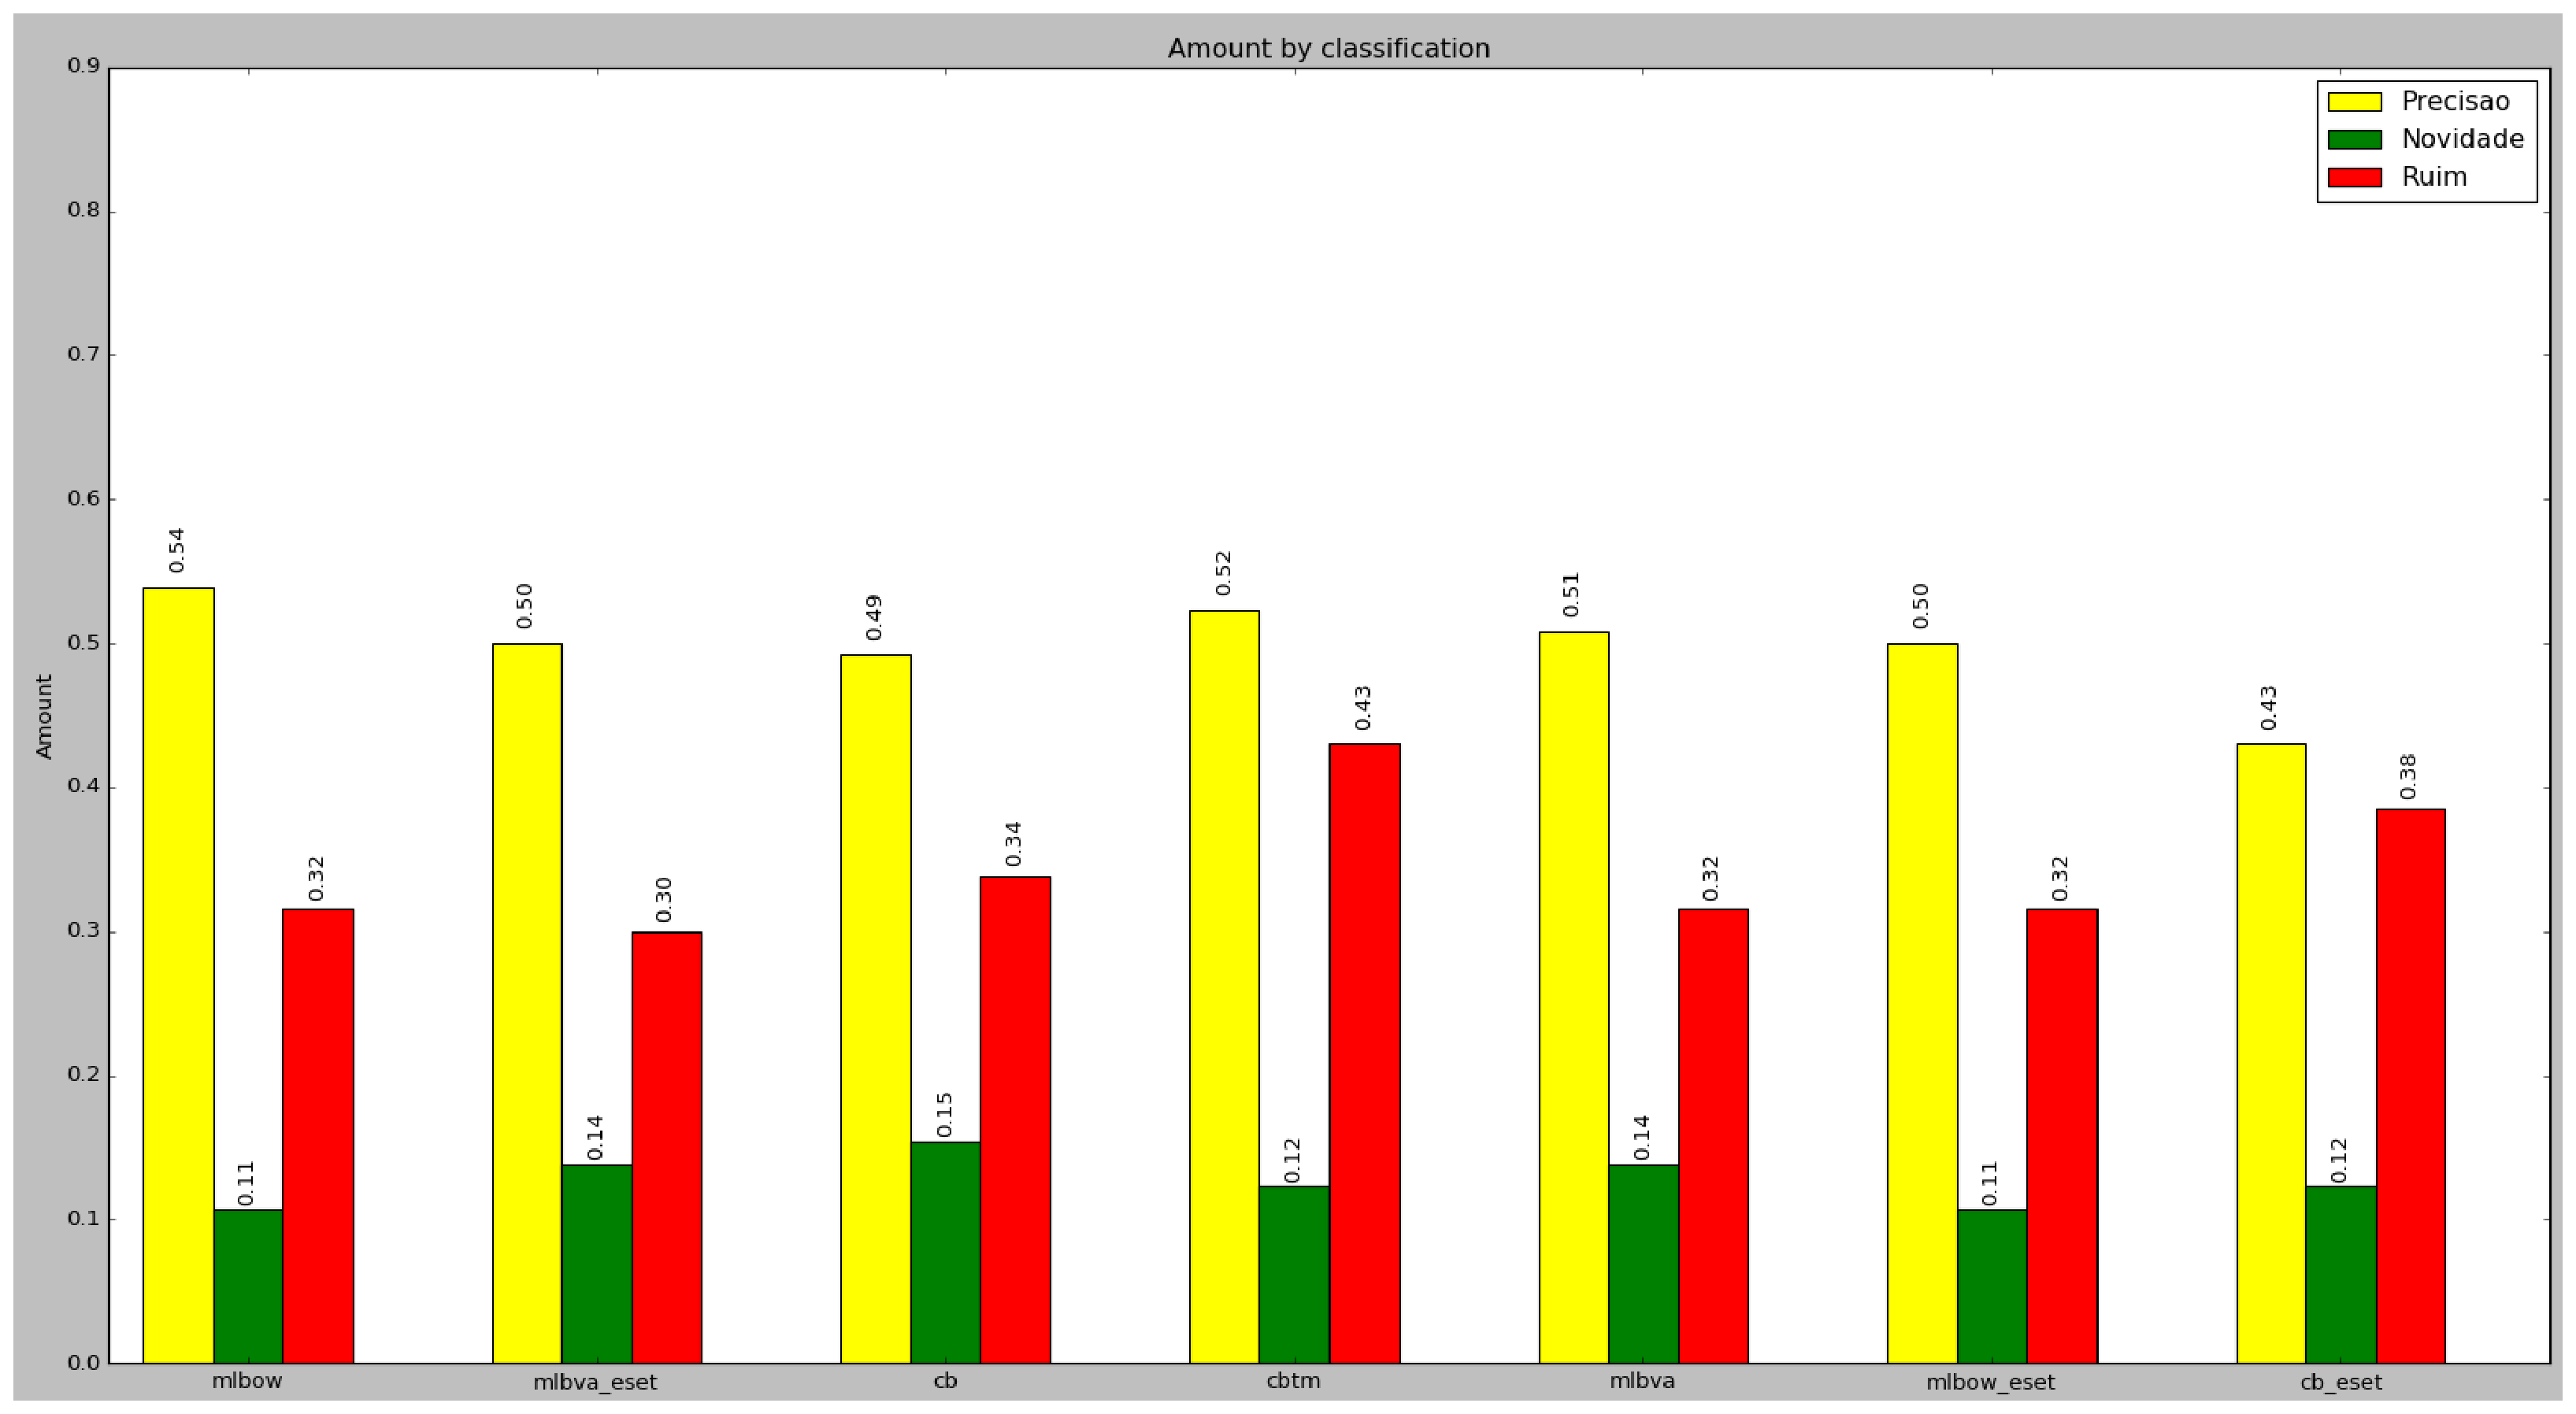
\includegraphics[width=0.9\textwidth]{figuras/metricas_segundo_experimento.eps}
  \caption{Métricas da segunda coleta de opinião}
  \label{fig:metricas_segundo_experimento}
\end{figure}

Pode-se ver pelo Gráfico \ref{fig:metricas_segundo_experimento} quanto a
precisão, o melhor resultado foi para estratégia \textit{mlbow}. Entretanto, a
melhora se deu em apenas 5\% em relação as estratégias baseadas em conteúdo do
\textit{AppRecommender}. Vale ressaltar também que a métrica \textbf{novidade}
mostra o que foi observado no Gráfico \ref{fig:segundo_experimento}, onde o
número de recomendações marcadas como surpresa se manteve estável entre as
ferramentas.

Além disso, pode-se perceber que a estratégia determinística com contexto
temporal \textit{cbtm} foi a que recomendou mais pacotes considerados ruins
pelo usuário, ou seja, a estratégia não atende aos requisitos. Isso difere dos
resultados encontrados na primeira coleta de opinião. Percebeu-se então que a mudança
no cálculo temporal favoreceu as estratégias de aprendizado de máquina, mas não
a determinística.

Sobre a questão de redundância, percebeu-se um problema quanto aos pacotes
instalados por outros gerenciadores de pacote. Por exemplo, caso o usuário seja
um programador ruby e tenha instalado pacotes ruby via \textit{apt} e
\textit{Ruby Version Manager} (rvm), o \textit{AppRecommender} pode recomendar
pacote instalados pelo \textit{rvm}, o que causa a redundância.

\begin{figure}[h]
  \centering
  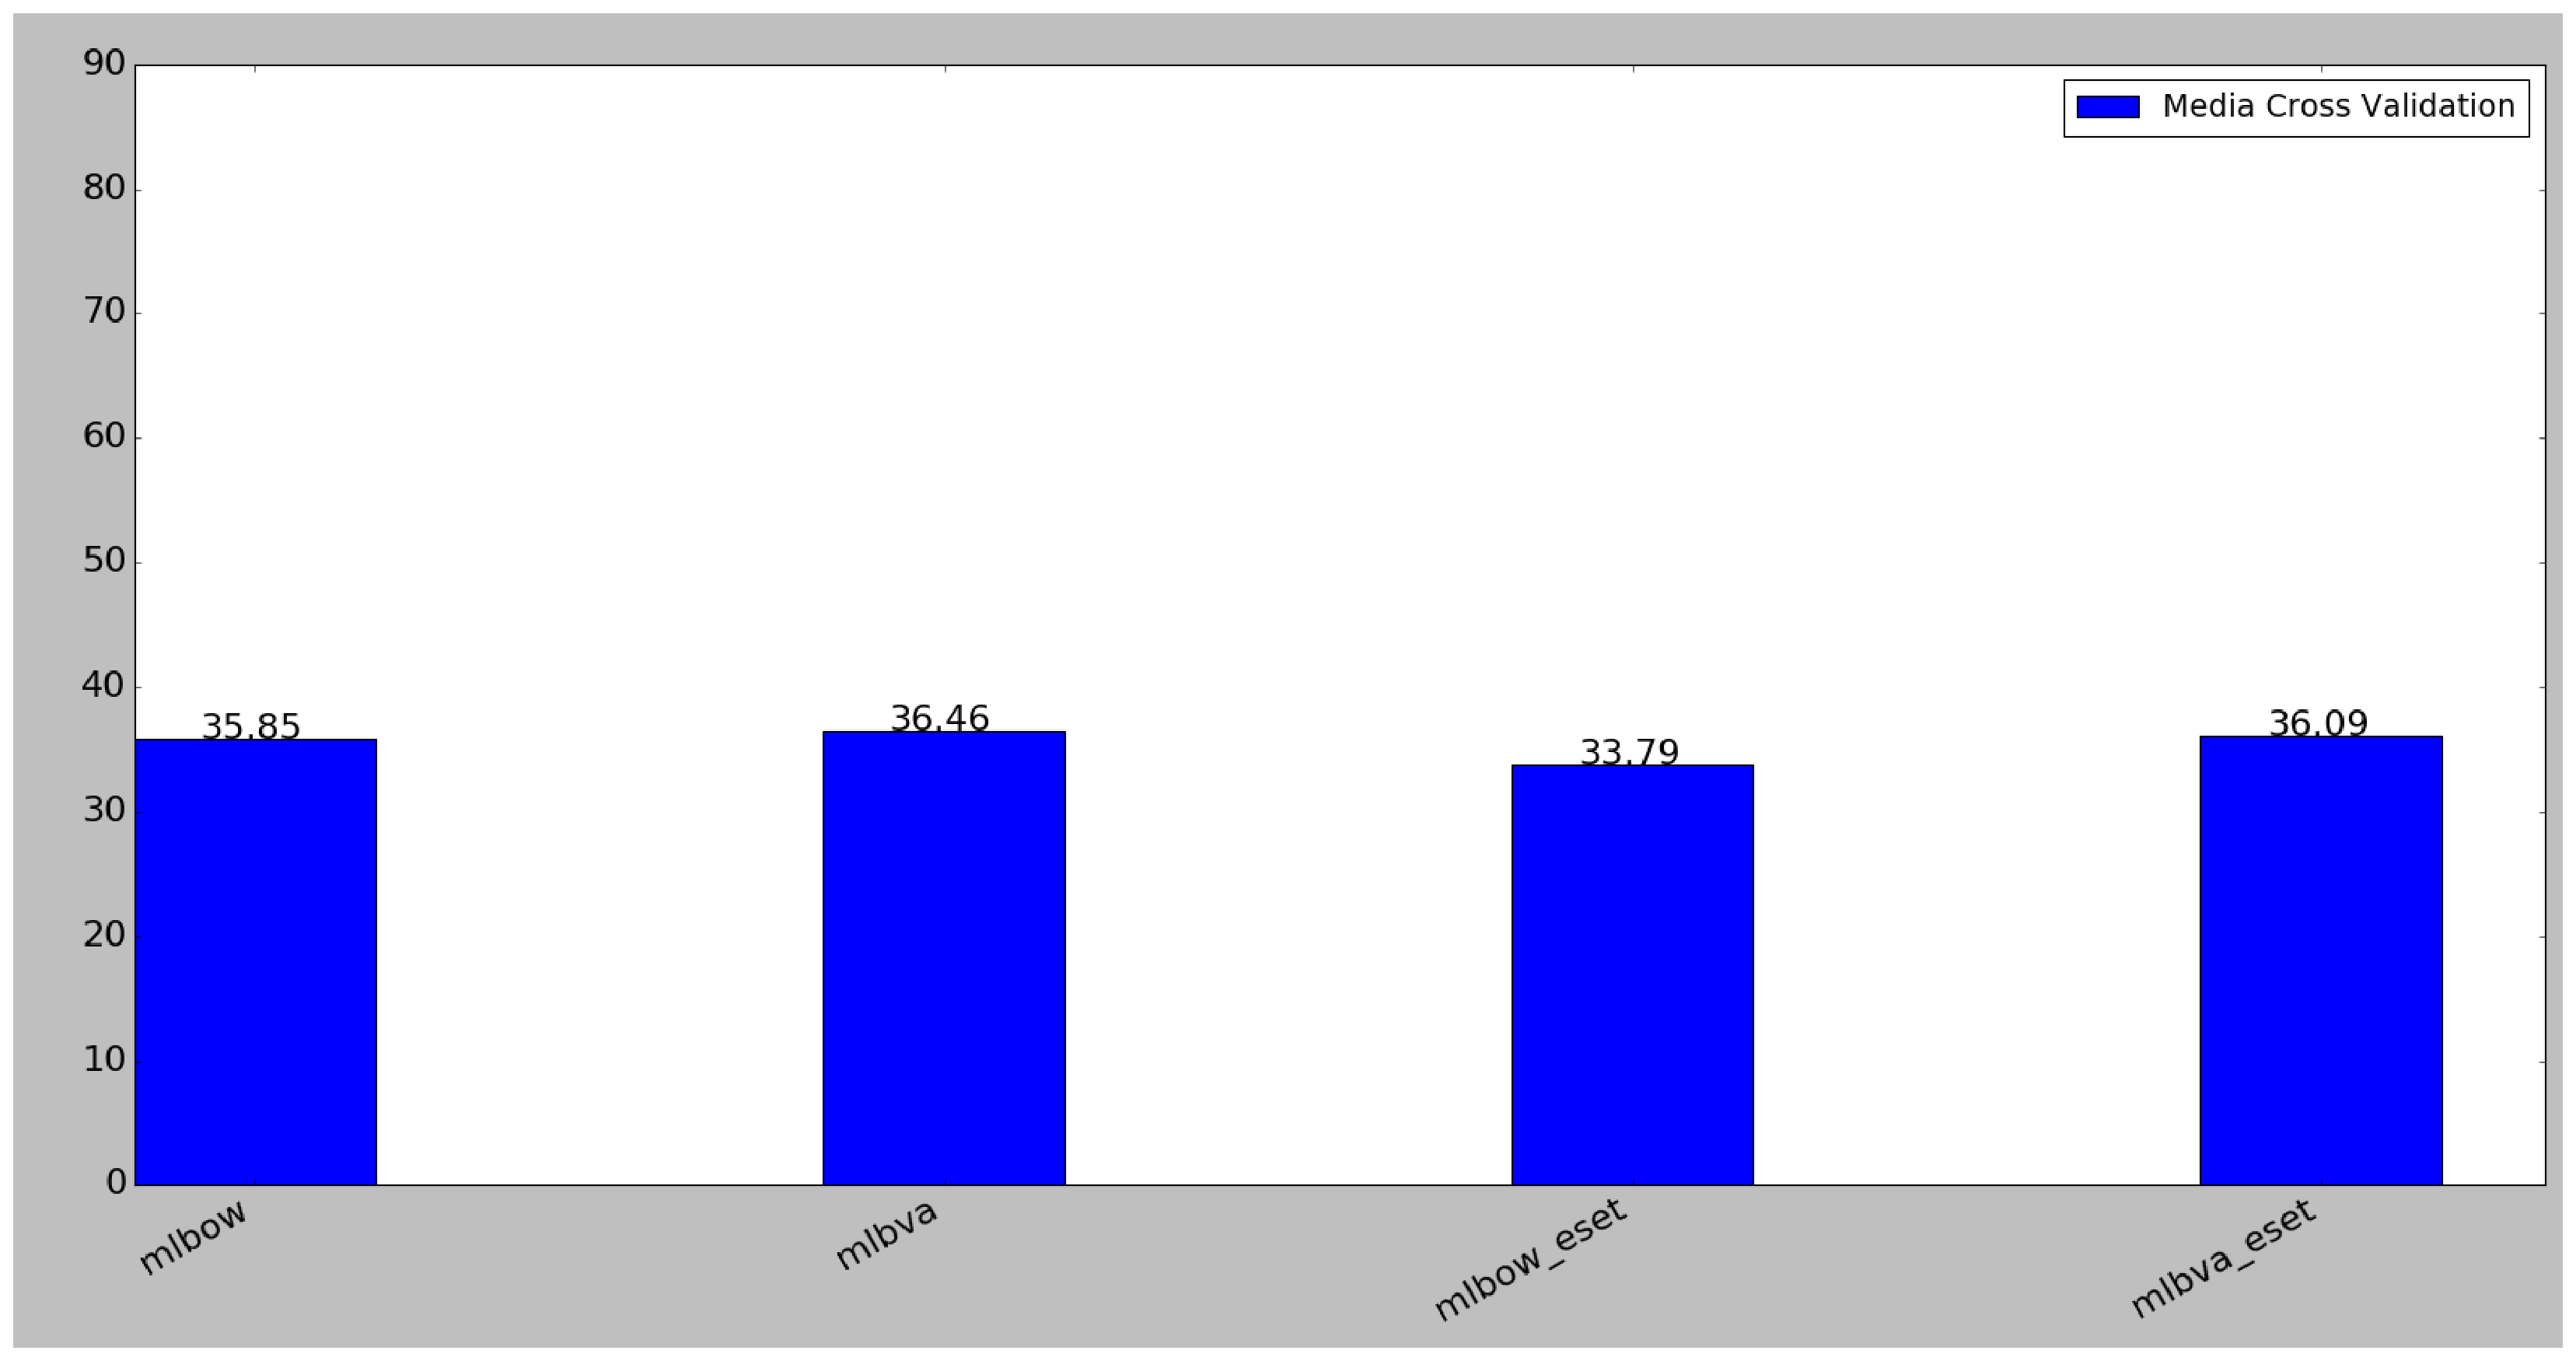
\includegraphics[width=0.9\textwidth]{figuras/segundo_experimento_cross_validation.eps}
    \caption{Métrica \textit{PorcentagemAcertos} obtida via cross validation para
    cada estratégia de aprendizado de máquina}
  \label{fig:segundo_experimento_cross_validation}
\end{figure}

Por fim, é necessário entender por que a melhoria encontrada foi de 3\%-5\% em
relação as estratégias baseadas em conteúdo já implementadas pelo
\textit{AppRecommender}. O gráfico da Figura \ref{fig:segundo_experimento_cross_validation}
mostra a média da métrica de acurácia \textit{PorcentagemAcertos}, definida na Seção
\ref{subsec:validacao_cruzada}, para cada estratégia de aprendizado de máquina.
Tal gráfico mostra que nenhuma estratégia teve uma média muito alta de acurácia,
sendo que acredita-se que a melhora encontrada por essas estratégias foi devido a
pré-filtragem de pacotes e não para a pós filtragem dos mesmos. Além disso, a
Tabela \ref{tab:resultados_p2} resume os resultados encontrados no segundo
experimento.

\begin{table}[]
    \centering
    \begin{tabular}{|l|l|l|l|}
        \hline
        & \textbf{Precisão} & \textbf{Novidade} & \textbf{Ruim} \\ \hline
        \textbf{mlbow}       & 0.54     & 0.11     & 0.32 \\ \hline
        \textbf{mlbva\_eset} & 0.50     & 0.14     & 0.30 \\ \hline
        \textbf{cb}          & 0.49     & 0.15     & 0.30 \\ \hline
        \textbf{cbtm}        & 0.52     & 0.12     & 0.43 \\ \hline
        \textbf{mlbva}       & 0.51     & 0.14     & 0.32 \\ \hline
        \textbf{mlbow\_eset} & 0.50     & 0.11     & 0.32 \\ \hline
        \textbf{cb\_eset}    & 0.43     & 0.12     & 0.38 \\ \hline
    \end{tabular}
    \caption{Resultados das métricas da segunda coleta de opnião}
    \label{tab:resultados_p2}
\end{table}

Vale ressaltar que mesmo com a estratégia de pré-filtragem sendo a que tenha
proporcionado a melhora nos resultados, pode-se ver que entre as estratégias de
aprendizado de máquina, as estratégias de classificação também tiveram influência
na melhoria dos resultados, pois todas as estratégias faziam a pré-filtragem de
forma idêntica, mas foi a \textit{mlbow} com o uso do \textit{Bag Of Words} e do
\textit{TFIDF} que apresentou os melhores resultados.

À partir dessa análise, acredita-se que um dos principais motivos para a baixa acurácia dos algoritmos
se dá pelo número de dados usado pelo treinamento. Em média, apenas 37 pacotes
estavam sendo usados para treinar o algoritmo, o que é uma
quantidade baixa para o treinamento do algoritmo propriamente dito.

Além disso, o método de aprendizado de máquina utilizado, o Bayes ingênuo pode
ser um método muito simples para entender a questão do gosto do usuário e seus
pacotes, sendo que outros métodos poderiam ter sido explorados.
